\documentclass{tufte-handout}
\title{SVT: One Pager\thanks{Thanks to MK, PEF}}
\author{Laurent Lathieyre}
% Settings
  %\date{28 March 2010} % without \date command, current date is supplied
  %\geometry{showframe} % display margins for debugging page layout
  % Load the packages
  \usepackage{graphicx} % allow embedded images
    \setkeys{Gin}{width=\linewidth,totalheight=\textheight,keepaspectratio}
    \graphicspath{{graphics/}} % set of paths to search for images
  \usepackage{amsmath}  % extended mathematics
  \usepackage{booktabs} % book-quality tables
  \usepackage{units}    % non-stacked fractions and better unit spacing
  \usepackage{multicol} % multiple column layout facilities
  \usepackage{lipsum}   % filler text
  \usepackage{fancyvrb} % extended verbatim environments
    \fvset{fontsize=\normalsize}  % default font size for fancy-verbatim environments
  \usepackage{glossaries}
    \setacronymstyle{long-short}
  

  % Standardize command font styles and environments
  \newcommand{\doccmd}[1]{\texttt{\textbackslash#1}}% command name -- adds backslash automatically
  \newcommand{\docopt}[1]{\ensuremath{\langle}\textrm{\textit{#1}}\ensuremath{\rangle}}% optional command argument
  \newcommand{\docarg}[1]{\textrm{\textit{#1}}}% (required) command argument
  \newcommand{\docenv}[1]{\textsf{#1}}% environment name
  \newcommand{\docpkg}[1]{\texttt{#1}}% package name
  \newcommand{\doccls}[1]{\texttt{#1}}% document class name
  \newcommand{\docclsopt}[1]{\texttt{#1}}% document class option name
  \newenvironment{docspec}{\begin{quote}\noindent}{\end{quote}}% command specification environment

\makeglossaries % Generate the glossary
\loadglsentries{defns}

\begin{document}
\maketitle % this prints the handout title, author, and date

\begin{abstract}
  \noindent
  this is my abstract
First use: \gls{svm}. Second use: \gls{svm}. \cite{toto2000}
\end{abstract}

\section{Business Environment}\label{sec:business-environment}
  \newthought{This is a limited snapshot of the current business environment} from a Market, Trends, Industry and Macroeconomics perspective.
  \begin{marginfigure}
    
\includegraphics{biz-env}
  \end{marginfigure}
  \subsection{Market Forces}\label{sec:market-forces}
  \subsection{Key Trends}\label{key-trends}
  \subsection{Industry Forces}\label{industry-forces}
  \subsection{Macroeconomics}\label{macroeconomics}



\section{Executive Summary}\label{exec-summary}
  \newthought{A brief overview that highlights the problem being addressed}, the proposed solution, and the anticipated impact. It provides a high-level understanding of the initiative.
  
\section{Customer Problem}\label{cust-pbm}
  \newthought{A clear and concise description of the pain points or challenges faced by customers} that the proposal aims to address. This section establishes the context for the proposed solution.

\section{Proposed Solution}\label{proposed-solution}
  \newthought{A detailed explanation of the product}, service, or idea being proposed, emphasizing how it directly addresses the customer problem identified earlier. It outlines the unique features, benefits, and value proposition of the solution.

\section{Target Market}\label{target-market}
  \newthought{An identification of the specific target market or customer segment} for the proposed solution. This section highlights the potential size and relevance of the target market.

\section{Competition}\label{Competition}
  \newthought{An analysis of existing competitors and alternative solutions} available in the market. It showcases how the proposed solution differentiates itself and offers superior value to customers.

\section{Key Metric}\label{key-metrics}
  \newthought{The metrics and performance indicators} used to measure the success and impact of the initiative. This section defines the goals and outcomes that will be tracked.

\section{Implementation Plan}\label{implementation-plan}
  \newthought{An outline of the steps, timeline, and resources} required to bring the proposal to fruition. It includes key milestones and considerations for successful execution.

\section{Risks and Mitigation}\label{risks-mitigation}
  \newthought{Identification and assessment of potential risks}, challenges, and obstacles that may arise during implementation. Strategies and contingency plans to mitigate these risks are also outlined.

\section{Conclusion}\label{Conclusion}
  \newthought{}





The Tufte-\LaTeX\ document classes define a style similar to the
style Edward Tufte uses in his books and handouts.  Tufte's style is known
for its extensive use of sidenotes, tight integration of graphics with
text, and well-set typography.  This document aims to be at once a
demonstration of the features of the Tufte-\LaTeX\ document classes
and a style guide to their use.

\section{Page Layout}\label{sec:page-layout}
\subsection{Headings}\label{sec:headings}
This style provides \textsc{a}- and \textsc{b}-heads (that is,
\Verb|\section| and \Verb|\subsection|), demonstrated above.

The Tufte-\LaTeX\ classes will emit an error if you try to use
\linebreak\Verb|\subsubsection| and smaller headings.

% let's start a new thought -- a new section
\newthought{In his later books},\cite{Tufte2006} Tufte
starts each section with a bit of vertical space, a non-indented paragraph,
and sets the first few words of the sentence in \textsc{small caps}.  To
accomplish this using this style, use the \Verb|\newthought| command:  
\begin{docspec}
  \doccmd{newthought\{In his later books\}, Tufte starts\ldots}
\end{docspec}

\subsection{Sidenotes}\label{sec:sidenotes}
One of the most prominent and distinctive features of this style is the
extensive use of sidenotes.  There is a wide margin to provide ample room
for sidenotes and small figures.  Any \Verb|\footnote|s will automatically
be converted to sidenotes.\footnote{This is a sidenote that was entered
using the \texttt{\textbackslash footnote} command.}  If you'd like to place ancillary
information in the margin without the sidenote mark (the superscript
number), you can use the \Verb|\marginnote| command.\marginnote{This is a
margin note.  Notice that there isn't a number preceding the note, and
there is no number in the main text where this note was written.}

The specification of the \Verb|\sidenote| command is:
\begin{docspec}
  \doccmd{sidenote[\docopt{number}][\docopt{offset}]\{\docarg{Sidenote text.}\}}
\end{docspec}

Both the \docopt{number} and \docopt{offset} arguments are optional.  If you
provide a \docopt{number} argument, then that number will be used as the
sidenote number.  It will change of the number of the current sidenote only and
will not affect the numbering sequence of subsequent sidenotes.

Sometimes a sidenote may run over the top of other text or graphics in the
margin space.  If this happens, you can adjust the vertical position of the
sidenote by providing a dimension in the \docopt{offset} argument.  Some
examples of valid dimensions are:
\begin{docspec}
  \ttfamily 1.0in \qquad 2.54cm \qquad 254mm \qquad 6\Verb|\baselineskip|
\end{docspec}
If the dimension is positive it will push the sidenote down the page; if the
dimension is negative, it will move the sidenote up the page.

While both the \docopt{number} and \docopt{offset} arguments are optional, they
must be provided in order.  To adjust the vertical position of the sidenote
while leaving the sidenote number alone, use the following syntax:
\begin{docspec}
  \doccmd{sidenote[][\docopt{offset}]\{\docarg{Sidenote text.}\}}
\end{docspec}
The empty brackets tell the \Verb|\sidenote| command to use the default
sidenote number.

If you \emph{only} want to change the sidenote number, however, you may
completely omit the \docopt{offset} argument:
\begin{docspec}
  \doccmd{sidenote[\docopt{number}]\{\docarg{Sidenote text.}\}}
\end{docspec}

The \Verb|\marginnote| command has a similar \docarg{offset} argument:
\begin{docspec}
  \doccmd{marginnote[\docopt{offset}]\{\docarg{Margin note text.}\}}
\end{docspec}

\subsection{References}
References are placed alongside their citations as sidenotes,
as well.  This can be accomplished using the normal \Verb|\cite|
command.\sidenote{The first paragraph of this document includes a citation.}

The complete list of references may also be printed automatically by using
the \Verb|\bibliography| command.  (See the end of this document for an
example.)  If you do not want to print a bibliography at the end of your
document, use the \Verb|\nobibliography| command in its place.  

To enter multiple citations at one location,\cite{Tufte2006,Tufte1990} you can
provide a list of keys separated by commas and the same optional vertical
offset argument: \Verb|\cite{Tufte2006,Tufte1990}|.  
\begin{docspec}
  \doccmd{cite[\docopt{offset}]\{\docarg{bibkey1,bibkey2,\ldots}\}}
\end{docspec}

\section{Figures and Tables}\label{sec:figures-and-tables}
Images and graphics play an integral role in Tufte's work.
In addition to the standard \docenv{figure} and \docenv{tabular} environments,
this style provides special figure and table environments for full-width
floats.

Full page--width figures and tables may be placed in \docenv{figure*} or
\docenv{table*} environments.  To place figures or tables in the margin,
use the \docenv{marginfigure} or \docenv{margintable} environments as follows
(see figure~\ref{fig:marginfig}):

\begin{marginfigure}%
  \includegraphics[width=\linewidth]{helix}
  \caption{This is a margin figure.  The helix is defined by 
    $x = \cos(2\pi z)$, $y = \sin(2\pi z)$, and $z = [0, 2.7]$.  The figure was
    drawn using Asymptote (\url{http://asymptote.sf.net/}).}
  \label{fig:marginfig}
\end{marginfigure}
\begin{Verbatim}
\begin{marginfigure}
  \includegraphics{helix}
  \caption{This is a margin figure.}
\end{marginfigure}
\end{Verbatim}

The \docenv{marginfigure} and \docenv{margintable} environments accept an optional parameter \docopt{offset} that adjusts the vertical position of the figure or table.  See the ``\nameref{sec:sidenotes}'' section above for examples.  The specifications are:
\begin{docspec}
  \doccmd{begin\{marginfigure\}[\docopt{offset}]}\\
  \qquad\ldots\\
  \doccmd{end\{marginfigure\}}\\
  \mbox{}\\
  \doccmd{begin\{margintable\}[\docopt{offset}]}\\
  \qquad\ldots\\
  \doccmd{end\{margintable\}}\\
\end{docspec}

Figure~\ref{fig:fullfig} is an example of the \Verb|figure*|
environment and figure~\ref{fig:textfig} is an example of the normal
\Verb|figure| environment.

\begin{figure*}[h]
  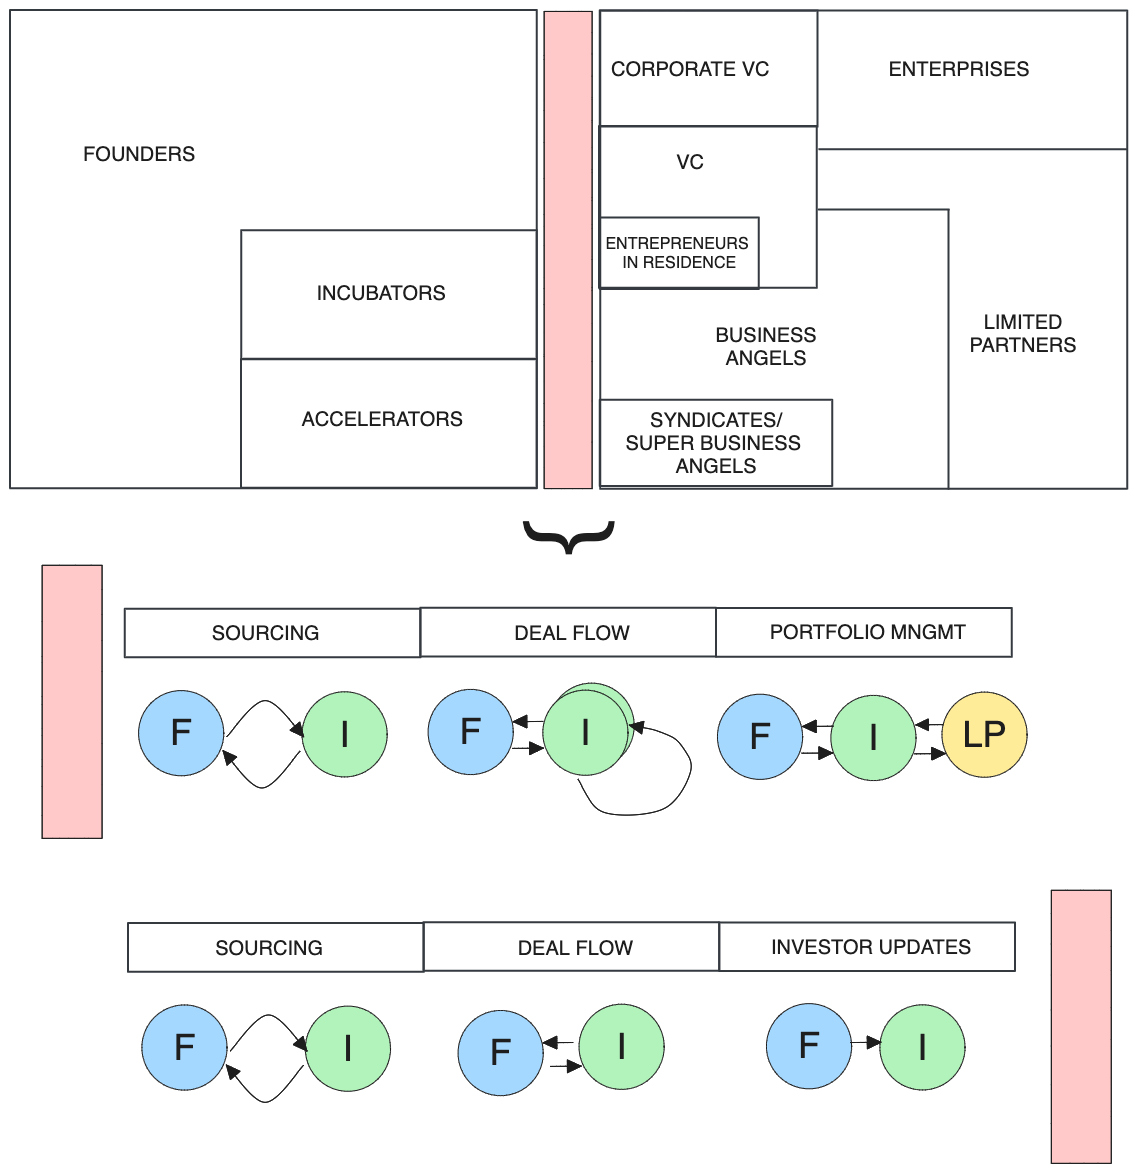
\includegraphics[width=\linewidth]{Fig-ecosystem-Drawing 2023-11-13 10.49.35.excalidraw.png}%
  \caption{The top diagram describes the two sides of the market. The bottom diagram describes the main workflows that 
  happen when demand meets supply.
  \emph{FNDRS: Founders, INCUB: Incubators, ACCEL: Accelerators, CVC: Corporate Venture Capital, VC: Venture Capital, 
  EIR: Entrepreneur In Residence, BA: Business Angel, LP: Limited Partner, SYN: Syndicate, SBA: Super Business Angel, 
  F: Founders, I: Investors, LP: Limited Partners.}}
  \label{fig:fullfig}%
\end{figure*}

% TODO add instructions for installing it globally




%\section{Acronyms}\label{sec:acronyms}
% Use the terms
%\gls{utc} is 3 hours behind \gls{adt} and 10 hours ahead of \gls{est}.
%utc is 3 hours be=hind adt
%\gls{rov} is smart.
%\gls{uuv} is better.
%\gls{xyz} is undefined.

%\section{Licenses}\label{sec:licenses}
%Typeset with the Tufte-\LaTeX\ packages is located at
%\url{https://github.com/Tufte-LaTeX/tufte-latex} with links to \smallcaps{svn} repository, mailing lists, bug tracker, and documentation.


% \bibliography{sample-handout}
% \bibliographystyle{plainnat}


\end{document}
